\section{Lemmas}
\label{app:sec:lemmas}
\begin{lemma}
\label{lemma:ica}
Let $\sbb \in \mathbb{R}^k$ and $\sbb'\in \mathbb{R}^k$ have independent components among which $g$ are Gaussian, and $P$ a rotation matrix such that $\sbb = P\sbb'$. Then, $P=\Pi^{-1} O \Pi'$ where $\Pi$ and $\Pi'$ are sign and permutation matrices such that the first $g$ components of $\Pi \sbb$ and $\Pi' \sbb'$ are Gaussian and $O$ is a block diagonal matrix such that $O^{(g)}$, the first $g \times g$ block of $O$, is orthogonal and the other block is identity.
\end{lemma}
\begin{proof}
  From~\cite{comon1994independent}, Theorem 10:
  Assume $\sbb = P\sbb'$, if the column $j$ of $P$ has more than one non-zero element then $s'_j$ is Gaussian. 
  
  Let us define permutations $\Pi_1$, $\Pi'_1$ such that the first $g$ components of $\Pi_1 \sbb$ and $\Pi'_1 \sbb'$ are Gaussian and $P_1  = \Pi_1 P (\Pi'_1)^{-1}$. We can see that $P_1$ is orthogonal.
  
[Omitted long matching line]
  \begin{align}
      &\begin{bmatrix} O_g & 0 \\ 0 & P_2 \end{bmatrix} = \Pi_1 P (\Pi'_1)^{-1} \\
      & \iff \begin{bmatrix} O_g & 0 \\ 0 & I \end{bmatrix} \begin{bmatrix} I & 0 \\ 0 & P_2 \end{bmatrix}  = \Pi_1 P (\Pi'_1)^{-1} \\
      & \iff \Pi_1^{-1} \begin{bmatrix} O_g & 0 \\ 0 & I \end{bmatrix} \begin{bmatrix} I & 0 \\ 0 & P_2 \end{bmatrix} \Pi'_1  = P
  \end{align}
  
  Therefore setting $\Pi' =   \begin{bmatrix} I & 0 \\ 0 & P_2 \end{bmatrix} \Pi'_1$ and $\Pi = \Pi_1$ and $O= \begin{bmatrix}O_g & 0 \\ 0 & I  \end{bmatrix}$ concludes the proof.
  
\end{proof}

\begin{lemma}
\label{lemma:eigdecomp}
Assume that Assumption 2 holds for $\Sigma_i$, and that there is an orthogonal matrix $P$ and diagonal matrices $\Sigma_i'$ such that for all $i$, $\Sigma_i' = P\Sigma_iP^{\top}$. Then, $P$ is a permutation matrix.
\end{lemma}
\begin{proof}
The proof is in two parts. First, we show that there exist some coefficients $\alpha_1, \dots, \alpha_m$ such that the matrix $\sum_i\alpha_i\Sigma_i$ has distinct coefficients on the diagonal. Then, since we have $\sum_i\alpha_i\Sigma'_i = P\left(\sum_i\alpha_i\Sigma_i\right)P^{\top}$, and the diagonal $\sum_i\alpha_i\Sigma_i$ has distinct entries, we can invoke the unicity of the eigenvalue decomposition for symmetric matrices, which shows that $P$ is necessarily a permutation matrix.
Now, the only thing left is to prove is that Assumption 2 implies the existence of this linear combination.

We assume by contradiction that any linear combination of the $\Sigma_i$ has two equal entries.

For $\alpha = [\alpha_1, \dots, \alpha_m]$, we let $\mathcal{S}(\alpha) = \diag(\sum_i\alpha_i\Sigma_i)\in\bbR^p$, where $\diag(\cdot)$ extracts the diagonal entries. The operator $\mathcal{S}$ is linear.
%
We now define for $j, j'\leq p$ the linear form $\ell_{jj'}(\alpha) = \mathcal{S}(\alpha)_j - \mathcal{S}(\alpha)_{j'}\in\bbR$. The assumption on the linear combinations of $\Sigma_i$ simply rewrites:
For all $\alpha\in\bbR^m$, there exists $j, j'\leq p$ such that $\ell_{jj'}(\alpha) = 0$.

From a set point of view, this relationship writes
$$
\bigcup_{j, j'}\mathrm{Ker}(\ell_{jj'}) = \bbR^m\enspace.
$$
Since the $\ell_{jj'}$ are all linear forms, the $\mathrm{Ker}(\ell_{jj'})$ are subspaces of dimensions $m$ or $m-1$, and since their union is of dimension $m$, there exists $j, j'$ such that  $\mathrm{Ker}(\ell_{jj'}) = \bbR^m$, i.e. such that $\ell_{jj'} = 0$.

As a consequence, we have for all $\alpha$, $\mathcal{S}(\alpha)_j = \mathcal{S}(\alpha)_{j'}$. This implies that the sequences $(\Sigma_{ij})_i$ and $(\Sigma_{ij'})_i$ are equal, which contradicts Assumption 2.


We have therefore shown that Assumption 2 implies the existence of a linear combination of the $\Sigma_i$ that has distinct entries, which concludes the proof.
\end{proof}


\begin{lemma}
\label{lemma:nonzerocoord}
Let us consider the following eigenvalue problem:
 \begin{align}
  & \begin{bmatrix} I + \Sigma_1 & I & \dots & I \\
    I & I + \Sigma_2 & \ddots & \vdots \\
    \vdots &  \ddots & \ddots & I  \\
    I & \dots & I  &I + \Sigma_m
  \end{bmatrix} \zb = \lambda \begin{bmatrix}
    I + \Sigma_1 & 0 & \dots  & 0 \\
    0 & I + \Sigma_2 & \ddots & \vdots \\
    \vdots & \ddots & \ddots & 0 \\
    0& \dots  & 0 &  I + \Sigma_m  \\
  \end{bmatrix} \zb
  \label{reducedeig}
\end{align}
where $\forall i, \enspace 1 \leq i \leq m, \enspace  \Sigma_m \in \bbR^{p, p}$ are positive diagonal matrices and I is the identity matrix.
If the first $p$ eigenvalues are distincts, the first $p$ eigenvectors $\zb^1, \dots, \zb^p, \zb^i \in \mathbb{R}^{mp}$ have different first non-zero coordinates.
\end{lemma}
%\bt{You implicitly assume that D is the block-diagonal part of C ?}
\begin{proof}
We sort the eigenvectors in $p$ groups of $m$ vectors so that all
vectors in group $l$ have their $l$-th coordinate
different from 0.
Let $\zb^{(l)}$ be an eigenvector in group $l$ and let us call $\wb_l \in
\mathbb{R}^{m}$ the non-zero coordinates of this eigenvector: $\forall i \in \{1 \dots m \}, w_{li} = z^{(l)}_{l + (i-1)p}$.

We have:
\begin{align}
\begin{bmatrix}
  1 + \Sigma_{1l} & 1 & \dots & 1  \\
  1 & 1 + \Sigma_{2l} & \ddots  &\vdots \\
  \vdots & \ddots & \ddots & 1  \\
  1 & \dots & 1 & 1 + \Sigma_{ml}  \\
\end{bmatrix} \wb_l =  \begin{bmatrix}
  1 + \Sigma_{1l} & 0 & \dots  & 0 \\
  0 & 1 + \Sigma_{2l} & \ddots & \vdots \\
  \vdots & \ddots & \ddots & 0 \\
  0& \dots  & 0 &  1 + \Sigma_{ml}  \\
\end{bmatrix} \wb_l \lambda_l
\label{eigsimp}
\end{align}

We now show that the biggest eigenvalue of~\eqref{eigsimp} is strictly above 1 while all
others are strictly below 1. The core of the proof comes from the study of the eigenvalues of a matrix modified by a rank 1 matrix. The reasoning we use here follows~\cite{golub1973some} (end of section 5).

Let us introduce 
$K^l = \diag(\Sigma_{1l} \dots \Sigma_{ml})$ and $\ub = \begin{bmatrix} 1 \\ \vdots \\ 1 \end{bmatrix}$.
Let us drop the index $l$ in the notations for simplicity.

The problem can be rewritten
\begin{align}
  &(\ub \ub^{\top} + K) \wb =  (I + K) \wb \lambda \\
  & \iff (I + K)^{-1}(\ub \ub^{\top} + K) \wb =   \wb \lambda
\end{align}

The characteristic polynomial is given by:
\begin{align}
  &\mathcal{P}(\lambda) = \det( (I + K)^{-1} K - \lambda I + (I + K)^{-1} \ub \ub^{\top}) \label{carpol} \\
  &\propto \det( I + ((I + K)^{-1} K - \lambda I)^{-1}(I + K)^{-1} \ub \ub^{\top})
\end{align}
where we implicitly focus here on eigenvalues $\lambda$ such that $\det((I + K)^{-1} K - \lambda I) \neq 0 \iff \forall i, \lambda \neq \frac{k_i}{1 + k_i}$.

We then use the following property:
Let $A \in \mathbb{R}^{a, b}$ and $B \in \mathbb{R}^{b, a}$ we have
$\det(I_a + AB) = \det(I_b + BA)$.

Let us call $\chi(\lambda) = \det( I + ((I + K)^{-1} K - \lambda I)^{-1}(I + K)^{-1} \ub \ub^{\top})$ we have:
\begin{align}
\chi(\lambda)
  &= 1 + \ub^{\top}((I + K)^{-1} K - \lambda I)^{-1}(I + K)^{-1} \ub \\
  &= 1  + \sum_{i=1}^m \frac1{1 + k_i} \frac1{ \frac{k_i}{1 + k_i} - \lambda}
\end{align}
%\bt{transition from (16) to (17) is not obvious to me !}
where $k_i = \Sigma_{il} > 0$.
% Since $k_i = \Sigma_{il} > 0$, the above secular function is simple to
% study.
% Let us re-order the values $\kappa_i = \frac{k_i}{1 + k_i}$ by increasing
% order $\kappa_1 < \dots < \kappa_m$. The eigenvalues $\lambda_i$ are such that
% $\kappa_1 < \lambda_1 < \kappa_2 < \lambda_2 < \kappa_3 < \dots < \kappa_m <
% \lambda_m$.
% Trivially $\kappa_m < 1$.
Taking the derivative we get 
\begin{align}
\chi'(\lambda) = \sum_{i=1}^m \frac1{1 + k_i} \frac1{ (\frac{k_i}{1 + k_i} - \lambda)^2} > 0
\end{align}

Trivially, $\forall i, \frac{k_i}{1 + k_i} < 1$. We also have
\begin{align}
  \chi(1) = 1 + \sum_{i=1}^{m} \frac1{1 + k_i} \frac1{ \frac{k_i}{1 + k_i} - 1} = 1 - m < 0
\end{align}
 and $\lim_{\lambda \rightarrow + \infty} \chi(\lambda) = 1$ so as $\chi$
 is continuous and strictly increasing on $[1, +\infty[$. Therefore, it reaches $0$ only once on this interval (excluding 1 since we know $\chi(1) \neq 0$). Therefore the greatest eigenvalue $\lambda^*$ is strictly above $1$ while all other eigenvalues are strictly below $1$.
 
  Note that because $\chi' > 0$, $\lambda^*$ is of multiplicity $1$. In the analysis above we ignored those eigenvalues $\lambda$ such that $\lambda = \frac{k_i}{1 + k_i}$ for some $i$. However since $\frac{k_i}{1 + k_i} < 1$, none of these eigenvalues can be the largest one.
 
 Finally, the $p$ first eigenvectors belong to different groups (the
 corresponding eigenvalues are all strictly above 1). This shows that these eigenvectors have
 different first non-zero coordinates. 
 
\end{proof}

% \begin{lemma}
% \label{lemma:rotation}
%   Let us consider the problem $(\Lambda + \delta
%   E)\ub = \ub \psi$ where $\Lambda = \diag(\lambda_1 \dots \lambda_{mp})$ is a diagonal matrix of positive values arranged in decreasing order, $\delta E = o(\lambda_p - \lambda_{p+1})$ and $\delta E = o(\lambda_{pm})$. The first eigenvectors $[\ub^1 \dots  \ub^p]$ are given by
%   $[\ub^1 \dots \ub^p] = [e_1 \dots e_p] \Theta + \delta Z$ where $e_i$ are the vectors of the canonical basis in $\bbR^{mp}$,
%   $\Theta \in \mathbb{R}^{p \times p}$ is a rotation matrix and $\delta Z =
%   O(\delta E)$
% \end{lemma}
% \begin{proof}
%   In matrix form denoting $\Psi = \diag(\psi_1 \dots \psi_{mp})$ the eigenvalues
%   in descending order and $U = [\ub^1 \dots \ub^{mp}]$ the matrix of associated
%   eigenvectors.
%   We want to solve
%   \begin{align}
%     (\Lambda +  \delta E)  U =  U \Psi
%   \end{align}
%   When the difference between any two values of $\Lambda$ is in $O(\min(\lambda_{pm}, \lambda_p - \lambda_{p+1}))$, no
%   rotation indeterminacy appears. We refer the reader to section 3.1 of the tutorial of~\cite{bamieh2020tutorial} to
%   have an explicit formula:
%   $U = I - \Pi \odot \delta E$
%   where $\odot$  is the Hadamar product and
%   $\Pi_{ij} = \begin{cases}
%     0 & \text{if } i =j \\
%     \frac1{\lambda_i - \lambda_j} & \text{if } i \neq i \\
%   \end{cases}$.

%   The rotation indeterminacy appears whenever the difference between two values
%   in $\Lambda$ is of the same order than $\delta E$. In which case we can
%   reparametrize the problem by:
%   \begin{align}
%     (\Lambda' +  \delta E')  U =  U \Psi
%   \end{align}
%   where $\Lambda'$ is obtained by replacing $\lambda_i$ by $\lambda_{i-1}$
%   whenever $\lambda_i - \lambda_{i-1} = O(\delta E)$ and the corresponding terms are
%   added in $\delta E'$ so that we always have $\Lambda + \delta E = \Lambda' +
%   \delta E'$ and $\delta E' = O(\delta E)$.

%   Let us assume without loss of generality that the $l$ first diagonal values of
%   $\Lambda'$ are the same while all others are different. Following derivations in~\cite{bamieh2020tutorial}, the
%   eigenvectors are given by:
%   \begin{align}
%     U = \Theta - \Theta \Pi' \odot \Theta^{\top}\delta E' \Theta
%   \end{align}
%   where $\Theta$ is a matrix such that its first $l, l$ block $\Theta^l$ diagonalizes the
%   first $l, l$ block of $\delta E'$, the off-diagonal blocks are nul and the
%   last diagonal block is identity.
%   \[
%     \Theta = \begin{bmatrix} \Theta^l & 0 \\ 0 & I_{km - l} \\ \end{bmatrix}
%   \]
%   and $\Pi'$ is given by
%   $\Pi'_{ij} = \begin{cases} 0 & \text{if } \lambda_i = \lambda_j \\
%     \frac1{\lambda_i - \lambda_j} & \text{if } \lambda_i \neq \lambda_j
%   \end{cases}$.
  
%   This can be rewritten:
%   \begin{align}
%       [\ub^1 \dots \ub^l] = [\eb_1 \dots \eb_l]\Theta^l
%       [\ub^{l+1} \dots \ub^{pm}] = [\eb_{l+1} \dots \eb_{pm}]
%   \end{align}
%   In particular we see that the eigenvectors are given up to a correction term by the canonical vectors with eigenvalues given (up to a correction term) by the diagonal values in $\Lambda$, but the ones that correspond to the same values of $\lambda_i$ up to $O(\delta_E)$ undergo a rotation $\Theta^l$ that depends on the sampling noise.
  
%   Note that as $\delta E = o(\lambda_p - \lambda_{p+1})$, none of the first $p$ eigenvectors can have the same eigenvalue as the last $pm -p$ up to $O(\delta E)$.
%   Therefore the first $p$ eigenvectors are given by the first $p$ canonical vectors of $\bbR^{pm}$ up to a rotation and a correction term: $[\ub^1 \dots \ub^p] = [e_1 \dots e_p]
%   \mathcal{O} + \delta Z$. Where $\mathcal{O} \in \bbR^{p, p}$ is a rotation and $\delta Z = O(\|\delta E \|_F^2)$.
% \end{proof}
% \bt{I'm lost between $\Theta$ and$ \mathcal{O}$}

\section{Identifiability results for $m< 3$}
\label{app:identifiability}
We have a slightly weaker identifiability result when $m=2$.
\begin{proposition}
  \label{prop:identifiability_2d}
  Let $m=2$, and suppose that the scalars $(1 + \Sigma_{1j})(1+\Sigma_{2j})$ for $j=1\dots p$ are all different. We let $\Theta'=(A_1', A_2', \Sigma_1',\Sigma_2')$ that also generates $\xb_1, \xb_2$. Then, there exists a permutation and scale matrix $P$ such that $A'_1 =A_1P$ and $A'_2 = A_2P^{-\top}$.
\end{proposition}
\begin{proof}
  We let $P=A_1^{-1}A_1'$. Since $C_{12} = I_p$, it holds 
  $A_2^{-1}A_2'= P^{-\top}$. Then, we have
  $I_p + \Sigma_1 = P(I_p + \Sigma'_1)P^{\top}$. This means that there exists $U\in\mathcal{O}_p$ such that $P = (I_p + \Sigma_1)^{\frac12}U(I_p + \Sigma'_1)^{-\frac12}$. Since $P^{-\top}(I_p+\Sigma'_2)P^{-1} = I_p+\Sigma_2$, we find
  $U(I_p+\Sigma'_1)(I_p+\Sigma'_2)U^{\top} = (I_p+\Sigma_1)(I_p+\Sigma_2)$. By identification, $U$ is a permutation matrix, and $P$ is a scale and permutation matrix.
\end{proof}
As a consequence, when there are only two subjects, it is possible to recover the components and noise levels up to a scaling factor.
%
When there is only one view, $m=1$, there is a global rotation indeterminacy: 
$
A_1(I_p + \Sigma_1)A_1^{\top} = A'_1(I_p + \Sigma_1){A'_1}^{\top}
$
for $A'_1 = A_1(I_p + \Sigma_1)^{\frac12}U(I_p + \Sigma_1)^{-\frac12}$ where $U$ is any orthogonal matrix. In this case, we lose identifiability.

% \section{Derivation of gradient and Hessian for the joint diagonalization}
% \label{app:jointdiag}
% We use a similar approach as\pierre{do we really need the orthogonal algorithm ? anyways, this should be put in appendix} in~\cite{ablin2018beyond} and optimize this loss using a quasi-newton approach. In our case though, we have to take into account the orthogonality constraint.
% In order to take into account orthogonality constraints, the gradient $G$ and Hessian $H$ are defined as 
% $\loss(\exp(\eps) O) = \loss(O) + \dotp{ \eps }{ G } + \dotp{ \eps }{ H \eps } + o(\|\eps \|_F^2)$ where $\eps$ is a small skew-symmetric matrix.

% Let us call $D^i = \mathcal{O} \hat{W}_i C_{ii} \hat{W}_i^{\top} \mathcal{O}^{\top}$ and notice that $D^i$ is symmetric.
% We have
% \begin{align}
%     &\loss(\exp(\eps) \mathcal{O}) \\
%     &= \loss((I + \eps + \frac12 \eps^2) \mathcal{O}) + o(\|\eps^2\|) \\
%     &= \frac1{2n} \sum_{i=1}^m \log \det \diag((I + \eps + \frac12 \eps^2) D^i(I + \eps + \frac12 \eps^2)^{\top}) + o(\|\eps^2\|) \\
%     &= \frac1{2n} \sum_{i=1}^m \log \det( \diag(D^i) + \diag(D^i \eps^{\top}) + \diag(\eps D^i) + \\ &\enspace \enspace \enspace \enspace \diag(\eps D^i \eps^{\top}) + \diag(\frac12 \eps^2 D^i) + \diag(\frac12 D^i (\eps^2)^{\top})) + o(\|\eps^2\|)\\
%     &= \frac1{2n} \sum_{i=1}^m \log \det( \diag(D^i) + 2\diag(\eps D^i) + \diag(\eps D^i \eps^{\top}) + 2\diag(\frac12 \eps^2 D^i)) + o(\|\eps^2\|)\\
%     &= \loss(\mathcal{O}) + \frac1{2n} \sum_{i=1}^m \log \det( I + 2\frac{\diag(\eps D^i)}{\diag(D^i)} + \frac{\diag(\eps D^i \eps^{\top})}{\diag(D^i)} + 2\frac{\diag(\frac12 \eps^2 D^i)}{\diag(D^i)}) + o(\|\eps^2\|) \\
%     &= \loss(\mathcal{O}) + \frac1{2n} \sum_{i=1}^m \tr \log( I + 2\frac{\diag(\eps D^i)}{\diag(D^i)} + \frac{\diag(\eps D^i \eps^{\top})}{\diag(D^i)} + 2\frac{\diag(\frac12 \eps^2 D^i)}{\diag(D^i)}) + o(\|\eps^2\|) \\
%     &= \loss(\mathcal{O}) + \frac1{2n} \sum_{i=1}^m \tr( 2\frac{\diag(\eps D^i)}{\diag(D^i)} + \frac{\diag(\eps D^i \eps^{\top})}{\diag(D^i)} \\ &\enspace \enspace \enspace \enspace + 2\frac{\diag(\frac12 \eps^2 D^i)}{\diag(D^i)} - 2(\frac{\diag(\eps D^i)}{\diag(D^i)})^2) + o(\|\eps^2\|) \\
%     &= \loss(\mathcal{O}) + \frac1{2n} \sum_{i=1}^m  \sum_k \left[ \sum_l 2\frac{\eps_{kl} D^i_{lk}}{D^i_{kk}} + \sum_{lm} \frac{\eps_{kl} D^i_{lm} \eps_{km}}{D^i_{kk}} \right.\\  &\left.\enspace \enspace \enspace \enspace + \sum_{lm}\frac{ \eps_{kl} \eps_{lm} D^i_{mk}}{D^i_{kk}} - 2\sum_{lm} \frac{ \eps_{kl}D^i_{lk} \eps_{km}D^i_{mk}}{(D^i_{kk})^2} \right] + o(\|\eps^2\|)
% \end{align}
% By identification we get
% \begin{align}
%     &G_{kl} = \frac1{n} \sum_i \frac{D^i_{lk}}{D^i_{kk}}
%     &H_{klmn} = \frac1{n} \sum_i (\delta_{km} \frac{D^i_{ln}}{D^i_{kk}} + \delta_{lm}\frac{D^i_{nk}}{D^i_{kk}} - 2 \delta_{km} \frac{D^i_{lk} D^i_{nk}}{(D^i_{kk})^2})
% \end{align}

% \begin{align}
%     &G_{kl} = \frac1{n} \sum_i \frac{D^i_{lk}}{D^i_{kk}}
%     &H_{klmn} = \frac1{n} \sum_i (\delta_{km} \frac{D^i_{ln}}{D^i_{kk}} + \delta_{lm}\frac{D^i_{nk}}{D^i_{kk}} - 2 \delta_{km} \frac{D^i_{lk} D^i_{nk}}{(D^i_{kk})^2})
% \end{align}
% We approximate the Hessian by replacing $D^i_{lk}$ by $D^i_{kk} \delta_{lk}$. This approximation is exact when the unmixed covariances are truly diagonal. The approximated Hessian is given by
% $\hat{H}_{klmn} = \frac1{n} \sum_i (\delta_{km} \delta_{ln} \frac{D^i_{ll}}{D^i_{kk}} + \delta_{lm} \delta_{kn} - 2 \delta_{kmln})$.
% Using the fact that $\eps$ is a skew-symmetric matrix

% Let us call $\hat{D^i} = \frac1{n} \sum_i D^i$.
% \begin{align}
% \dotp{ G }{ \eps } + \frac12 \dotp{ \eps }{ \hat{H} \eps } &= \sum_{kl} \eps_{kl} G_{kl} + \frac12 \sum_{klmn} \hat{H}_{klmn} \eps_{kl} \eps_{mn} \\
% &= \sum_{kl} G_{kl} \eps_{kl} + \frac12 \left[\sum_{kl} \frac{\hat{D}^i_{ll}}{\hat{D}^i_{kk}} \eps_{kl}^2 + \sum_{kl}\eps_{kl} \eps_{lk} - 2\sum_k \eps_{kk} \right]
% \end{align}
% Using the fact that $\eps$ is anti-symmetric gives:
% \begin{align}
% \dotp{ G }{ \eps } + \dotp{ \eps }{ \hat{H} \eps }
% &= \sum_{k} \sum_{l < k} (G_{kl} - G_{lk}) \eps_{kl} + \frac12(\sum_{k} \sum_{l < k} (\frac{\hat{D}^i_{ll}}{\hat{D}^i_{kk}} + \frac{\hat{D}^i_{kk}}{\hat{D}^i_{ll}}) \eps_{kl}^2 -\sum_{k} \sum_{l < k}2\eps_{kl}^2) \\
% &= \sum_{k} \sum_{l < k} (G_{kl} - G_{lk}) \eps_{kl} + \frac12(\sum_{k} \sum_{l < k} \left[\frac{\hat{D}^i_{ll}}{\hat{D}^i_{kk}} + \frac{\hat{D}^i_{kk}}{\hat{D}^i_{ll}} - 2\right] \eps_{kl}^2)
% \end{align}
% So updates are given by
% $\mathcal{O} \leftarrow \exp(J) \mathcal{O}$ where $J_{kl} = \frac{G_{kl} - G_{lk}}{\frac{\hat{D}^i_{ll}}{\hat{D}^i_{kk}} + \frac{\hat{D}^i_{kk}}{\hat{D}^i_{ll}} - 2}$.


% \section{Derivation of log-likelihood}
% \label{likelihood_derivation}


% and the log-likelihood writes:
% \begin{align}
%   \mathcal{L} = &\sum_{i=1}^m\left(-\log|W_i| + \frac12 \log |\Sigma_i|\right) + \frac12 \log(|\sum_{i=1}^m \Sigma_i^{-1} + I|) + \frac12 (\sum_{i=1}^m \dotp{ \yb_i }{ \Sigma_i^{-1} \yb_i } \\&  - \frac12 \dotp{ \left(\sum_{i=1}^m \Sigma_i^{-1} + I \right)^{-1} \sum_{i=1}^m \left(\Sigma_i^{-1} \yb_i \right) }{ \sum_{i=1}^m \left(\Sigma_i^{-1} \yb_i \right) })
% \end{align}
% which yields the expected formula.

\section{EM E-step and M-step for ShICA with Gaussian components}
  \subsection{E-step}
  \label{conditional_density}
  The derivations are the same as in section~\ref{app:emestep1} but the sum over
  $\alpha \in {\frac12, \frac32}$ is replaced by just $\alpha=1$.


\subsection{M-step}
The function to minimize in the M-step is then given by:
\begin{align}
  \Jcal &= -\log p(\xb, \sbb) \\
        &= \sum_{i=1}^m \log(|\Sigma_i|) + \\ &\enspace \enspace \enspace \frac12 \tr(\Sigma_i^{-1} \left[(\yb_i - \EE[\sbb | \xb]) (\yb_i - \EE[\sbb | \xb])^{\top}+ \VV[\sbb | \xb]\right]) \\ &\enspace \enspace \enspace + c
\end{align}
where $c$ does not depend on $\Sigma_i$

Therefore we get closed-form updates for $\Sigma_i$: 
\begin{align}
\Sigma_i \leftarrow  \diag((\yb_i - \EE[\sbb | \xb]) (\yb_i - \EE[\sbb | \xb])^{\top}+ \VV[\sbb | \xb])
\end{align}
Plugging in the closed-form formula for $\EE[\sbb|\xb]$ and $\VV[\sbb|\xb]$ we get updates that only depends on the covariances $\hat{C_{ij}} = \EE[\xb_i \xb_j^{\top}]$.
\begin{align*}
\Sigma_i \leftarrow &\diag(\hat{C_{ii}} \\&- 2 \VV[\sbb | \xb]  \sum_{j=1}^m \Sigma_j^{-1} \hat{C}_{ji}  \\&+ \VV[\sbb | \xb]  \sum_{j = 1}^m \sum_{l = 1}^m \left(\Sigma_j^{-1} \hat{C}_{jl} \Sigma_l^{-1} \right) \VV[\sbb | \xb] \\&+ \VV[\sbb | \xb])
\end{align*}


\section{EM E-step and M-step for ShICA with non-Gaussian components}
\label{app:emestep}

  \subsection{E-step}
  \label{app:emestep1}
  The complete likelihood is given by
\begin{align}
  p(\xb, \sbb) &= \prod_i p(\xb_i | \sbb) p(\sbb) \\
  &= \prod_i p(\xb_i | \sbb) \prod_j \sum_{\alpha \in \{0.5, 1.5\}}p(s_j | \alpha) \\
\end{align}
where 
\begin{align}
  p(s_j | \alpha) = \Ncal(s_j; 0, \alpha)
\end{align}

We have
\begin{align}
  p(\xb_i | \sbb) &=|W_i|\Ncal(\yb_i; \sbb, \Sigma_i)  \\
                  &= |W_i| \prod_j \Ncal(y_{ij}; s_j, \Sigma_{ij})
\end{align}
where $\Sigma_{ij}$ is the coefficient $j, j$ of $\Sigma_i$ and $\yb_i = W \xb_i$.

Let us introduce a first lemma:
\begin{lemma}
  \label{lemma:multmgauss}
  \begin{align*}
    \prod_{i=1}^m \Ncal(x_i; u, v_i) = \prod_{i=1}^m \Ncal(x_i; \bar{x}, v_i) \sqrt{2 \pi \bar{v}} \Ncal(\bar{x}; u, \bar{v})
  \end{align*}
  where $\bar{v} = (\sum_{i=1}^m v_i^{-1})^{-1}$ and $\bar{x} = \frac{\sum_i v_i^{-1}
    x_i}{\sum_i v_i^{-1}}$.
\end{lemma}
\begin{proof}
  We have that
  \begin{align}
    \frac1{v_i}(x_i - u)^2 &= \frac1{v_i}(x_i - u)^2 \\
                           &=\frac1{v_i}(x_i - \bar{x} + \bar{x} - u)^2 \\
                           &=\frac1{v_i}(x_i - \bar{x})^2 + \frac1{v_i}(\bar{x} - u)^2 \label{eq:lem:multigauss}
  \end{align}
  and therefore
  \begin{align}
    &\prod_i \frac1{\sqrt{2 \pi v_i}}\exp(-\frac1{2v_i}(x_i - \mu)^2) \\
    &= \prod_j \frac1{\sqrt{2 \pi v_i}}\exp(-\frac12 (\frac1{v_i}(x_i - \bar{x})^2 + \frac1{v_i}(\bar{x} - u)^2)) \\ 
    &= \prod_j \Ncal(x_i, \bar{x}, v_i) \exp(-\frac12( \sum_i \frac1{v_i})(\bar{x} - u)^2)) \\ 
  \end{align}
    so the desired result follow.
\end{proof}

By Lemma~\ref{lemma:multmgauss}, we have
\begin{align}
  \prod_i p(\xb_i | \sbb) &= \prod_i |W_i| \prod_j \Ncal(y_{ij}; \bar{y}_{j}, \Sigma_{ij}) \sqrt{2 \pi \bar{\Sigma_{j}}} \Ncal(\bar{y}_j; s_j, \bar{\Sigma_{j}})  \\
\end{align}
where $\bar{y}_j = \frac{\sum_i \Sigma_{ij}^{-1} y_{ij}}{ \sum_i
  \Sigma_{ij}^{-1}}$ and $\bar{\Sigma_{j}} = (\sum_i
\Sigma_{ij}^{-1})^{-1}$.
Hiding variable that do not depend on $\sbb$ we obtain

\begin{align}
  \prod_i p(\xb_i | \sbb) &\propto \prod_j \Ncal(\bar{y}_j; s_j, \bar{\Sigma_{j}})  \\
\end{align}

Then we get
\begin{align}
  p(\xb, \sbb) &= \prod_j \sum_{\alpha \in \{0.5, 1.5\}} \Ncal(s_j; \bar{y}_j, \bar{\Sigma_{j}}) \Ncal(s_j; 0, \alpha)
\end{align}

Let us now prove a second Lemma:
\begin{lemma}
  \label{lemma:multgauss}
  \begin{align*}
    \mathcal{N}(x; y, \nu) \mathcal{N}(x, 0, \alpha) = \mathcal{N}(y; 0, \nu + \alpha) \mathcal{N}(x; \frac{\alpha y}{\alpha + \nu}, \frac{\nu \alpha}{\alpha + \nu})
  \end{align*}
\end{lemma}
\begin{proof}

  We have 
\begin{align}
  &\mathcal{N}(x; y, \nu) \mathcal{N}(x, 0, \alpha) = \frac{\exp \left(-\frac{(x-y)^2}{2\nu} \right)}{\sqrt{2 \pi \nu}} \frac{\exp \left(-\frac{x^2}{2\alpha}\right)}{\sqrt{2 \pi \alpha}}
\end{align}

Then,
\begin{align}
  &\exp \left(-\frac{(x-y)^2}{2\nu} \right) \\
  &= \exp\left(- \frac{\alpha (x-y)^2 + \nu x^2}{2 \alpha \nu} \right) \\
  &= \exp\left(- \frac{\alpha (x^2 -2xy + y^2) + \nu x^2}{2 \alpha \nu} \right) \\ 
  &=\exp\left(- \frac{x^2(\alpha + \nu) -2x(\alpha y) + \alpha y^2 }{2 \alpha \nu} \right) \\
  &= \exp\left( -\frac{x^2 -2x\frac{\alpha y}{\alpha + \nu} + \frac{\alpha y^2}{\alpha + \nu} }{2 \frac{\alpha \nu}{\alpha + \nu}} \right) \\
  &= \exp\left( -\frac{(x - \frac{\alpha y}{\alpha + \nu})^2 - ( \frac{\alpha y}{\alpha + \nu} )^2 + \frac{\alpha y^2}{\alpha + \nu} }{2 \frac{\alpha \nu}{\alpha + \nu}} \right) \\
  &= \exp\left( -\frac{(x - \frac{\alpha y}{\alpha + \nu})^2}{2\frac{\alpha \nu}{\alpha + \nu}}\right) \exp \left(-\frac{ - \alpha^2 y^2 + (\alpha + \nu)\alpha y^2 }{2 \alpha \nu(\alpha + \nu)} \right) \\
  &= \exp\left( -\frac{(x - \frac{\alpha y}{\alpha + \nu})^2}{2\frac{\alpha \nu}{\alpha + \nu}}\right) \exp \left(-\frac{\nu\alpha y^2 }{2 \alpha \nu(\alpha + \nu)} \right)
\end{align}

and
\begin{align}
  \frac1{\sqrt{2 \pi \nu}\sqrt{2 \pi \alpha}} &= \frac1{\sqrt{2 \pi (\nu + \alpha)}\sqrt{2 \pi \frac{\nu \alpha}{\nu + \alpha}}}
\end{align}
so that the desired result follow.
\end{proof}
                 
By Lemma~\ref{lemma:multgauss}, we have:
\begin{align}
  &p(\xb, \sbb) \\
  &= \prod_j \sum_{\alpha \in \{0.5, 1.5\}} \Ncal(\bar{y}_{j}; 0 , \bar{\Sigma}_{j} + \alpha) \Ncal(s_j; \frac{\alpha \bar{y}_{j}}{\alpha + \bar{\Sigma_{j}}}, \frac{\bar{\Sigma_{j}}\alpha}{\alpha + \bar{\Sigma_{j}}})
\end{align}

and therefore we get:
\begin{align}
  p(\sbb | \xb) &= \frac{p(\sbb, \xb)}{\int_{\sbb} p(\sbb, \xb)} \\
                &= \prod_j \frac{\sum_{\alpha \in \{0.5, 1.5\}} \theta_{\alpha} \Ncal(s_j; \frac{\alpha \bar{y}_{j}}{\alpha + \bar{\Sigma_{j}}}, \frac{\bar{\Sigma_{j}}\alpha}{\alpha + \bar{\Sigma_{j}}})}{\sum_{\alpha \in \{0.5, 1.5\}} \theta_{\alpha}}
\end{align}
where $\theta_{\alpha} = \Ncal(\bar{y}_{j}; 0 , \bar{\Sigma}_{j} + \alpha)$.

So we obtain the desired result:
\begin{align}
  &\EE[s_j | \xb] = \frac{\sum_{\alpha \in \{0.5, 1.5\}} \theta_{\alpha} \frac{\alpha \bar{y}_{j}}{\alpha + \bar{\Sigma_{j}}}}{\sum_{\alpha \in \{0.5, 1.5\}} \theta_{\alpha}} \\
  & \VV[s_j | \xb] = \frac{\sum_{\alpha \in \{0.5, 1.5\}} \theta_{\alpha} \frac{\bar{\Sigma_{j}}\alpha}{\alpha + \bar{\Sigma_{j}}}}{\sum_{\alpha \in \{0.5, 1.5\}} \theta_{\alpha}}  
\end{align}

\subsection{M-step}
The function to minimize in the M-step is then given by:
\begin{align}
  \Jcal &= -\log p(\xb, \sbb) \\
  &= \sum_{i=1}^m - \log(|W_i|) + \log(|\Sigma_i|) + \\& \enspace \enspace \frac12 \tr(\Sigma_i^{-1} \left[(\yb_i - \EE[\sbb | \xb]) (\yb_i - \EE[\sbb | \xb])^{\top}+ \VV[\sbb | \xb]\right]) + c
\end{align}
where $c$ does not depend on $\Sigma_i$ or $W_i$

Therefore we get closed-form updates for $\Sigma_i$: 
\begin{align}
\Sigma_i \leftarrow  \diag((\yb_i - \EE[\sbb | \xb]) (\yb_i - \EE[\sbb | \xb])^{\top}+ \VV[\sbb | \xb])
\end{align}

% and the approximated Hessian $\widehat{\mathcal{H}^{W_i}}$
We update $W_i$ by performing a quasi-Newton step. 
% The gradient $\mathcal{G}^{W_i}$, the Hessian $\mathcal{H}^{W_i}$  are given by
% $\mathcal{G}((I + \epsilon)W_i) = C(W_i) + \dotp{ \epsilon }{ \mathcal{G}^{W_i} } +
% \frac12 \dotp{ \epsilon }{ \mathcal{H}^{W_i} \epsilon }$ so
% \begin{align*}
%   &\mathcal{G}^{} = -I + (\Sigma_i)^{-1}(\yb_i - \mathbb{E}[\sbb|\xb])(\yb_i)^{\top} , \enspace \mathcal{H}^{W_i}_{a, b, c, d} = \delta_{a, c} \frac{y_{ib} y_{id}}{\Sigma_i_a}, \enspace \widehat{\mathcal{H}^{W_i}_{a, b, c, d}} =  \delta_{a, c} \delta_{b, d}\frac{(y_{ib})^2}{\Sigma_i_a}
% \end{align*}
% where the Hessian approximation is exact when the unmixed data have truly independent components.

We use the relative gradient $\mathcal{G}^{W_i}$ and $\mathcal{H}^{W_i}$ defined
by
\begin{align}
\mathcal{J}(W_i + \varepsilon W_i) = \mathcal{J}(W_i) + \dotp{ \varepsilon}{\mathcal{G}^{W_i}} + \frac12 \dotp{ \varepsilon}{\mathcal{H}^{W_i} \varepsilon }
\end{align}

 We get:
 \begin{align}
   \mathcal{J}(W_i + \varepsilon W_i) &= \sum_{i=1}^m \bigg[ -\log(|W_i|) -\log(|I_k + \varepsilon|) \nonumber \\&- \log(\mathcal{N}(\yb_i + \varepsilon \yb_i; \sbb; \Sigma_i)) \bigg] + const \\
                                      &= \mathcal{J}(W_i) - \tr(\varepsilon) + \frac12 \tr(\varepsilon^2) \nonumber \\& \enspace \enspace + \frac12 \bigg[\dotp{ \varepsilon \yb_i}{ (\Sigma_i)^{-1} (\yb_i - \sbb) } + \nonumber \\& \enspace \enspace \dotp{ (\yb_i - \sbb)}{ (\Sigma_i)^{-1} \varepsilon \yb_i } + \dotp{ \varepsilon \yb_i}{ (\Sigma_i)^{-1} \varepsilon \yb_i } \bigg] \nonumber \\ & \enspace + o(\|\varepsilon\|^2) \\
                                      &= \mathcal{J}(W_i) - \sum_a \varepsilon_{a, a} + \frac12 \sum_{a, b} \varepsilon_{a,b} \varepsilon_{b, a} \nonumber \\& \enspace \enspace + \sum_{a, b} \varepsilon_{a, b} \left[(\Sigma_i)^{-1}(\yb_i - \sbb) (\yb_i)^{\top} \right]_{a, b} \nonumber \\& \enspace \enspace + \frac12 \sum_{a, b} \varepsilon_{a, b} \left[(\Sigma_i)^{-1} \varepsilon \yb_i (\yb_i)^{\top}\right]_{a, b} \nonumber \\ & \enspace + o(\|\varepsilon\|^2) \\
                                      &= \mathcal{J}(W_i) - \sum_a \varepsilon_{a, a} + \frac12 \sum_{a, b} \varepsilon_{a,b} \varepsilon_{b, a} \nonumber \\& \enspace \enspace + \sum_{a, b} \varepsilon_{a, b} \left[(\Sigma_i)^{-1}(\yb_i - \sbb) (\yb_i)^{\top} \right]_{a, b} + \nonumber \\& \enspace \enspace \frac12 \sum_{a, b, d} \varepsilon_{a, b} (\Sigma_i)^{-1}_{a, a} \varepsilon_{a, d} \left[\yb_i (\yb_i)^{\top}\right]_{d, b} \nonumber \\ & \enspace + o(\|\varepsilon\|^2)
 \end{align}

 So:
 \begin{equation}
 \mathcal{G}^{W_i}_{a, b} =  -\delta_{a,b} + \left[(\Sigma_i)^{-1} (\yb_i - \sbb)(\yb_i)^{\top}\right]_{a, b}
 \end{equation}
 and
 \begin{equation}
 \mathcal{H}^{W_i}_{a, b, c, d} = \delta_{a, d}\delta_{b, c} + \delta_{a, c} \frac{y_{ib} y_{id}}{\Sigma_{ia}}
 \end{equation}
 
 We approximate the Hessian by
 \begin{align}
 \widehat{\mathcal{H}^{W_i}_{a, b, c, d}} = \delta_{ad} \delta_{bc} + \delta_{ac} \delta_{bd}\frac{(y_{ib})^2}{\Sigma_{ia}}
\end{align}
where the Hessian approximation is exact when the unmixed data have truly independent components.

Updates for $W_i$ are then given by
$W_i \leftarrow (I - \rho (\widehat{\mathcal{H}^{W_i}})^{-1} \mathcal{G}^{W_i}) W_i$, 
where $\rho$ is chosen by backtracking line-search.
We alternate between computing the statistics $\mathbb{E}[\sbb|\xb]$ and
$\Var[\sbb|\xb]$ (E-step) and updates of parameters $\Sigma_i$ and $W_i$ for $i=1 \dots m$ (M-step).




% \begin{figure}
%   \includegraphics[width=0.5\textwidth]{./figures/synthetic_Gaussian_source_50_samples.pdf}
% \end{figure}

\section{CamCAN spatial maps}
\label{app:shica:maps}
We use $m=496$ subjects and fit ShICA-ML with $p=10$ components. We localize the
components of each subject using sLORETA~\cite{pascual2002standardized}. Then
components are registered to a common brain and averaged. Thresholded maps are
displayed below along with the time courses of each component. Spatial maps obtained with ShICA-ML highlight the ventral visual cortex and auditive cortex. The results suggest that the response of the auditive cortex is faster and lasts a shorter time than the response of the ventral visual cortex.


% In contrast, maps obtained with CanICA are very similar and miss the activation in the auditory cortex.
% \subsubsection{Components obtained with ShICA-ML}
{\centering
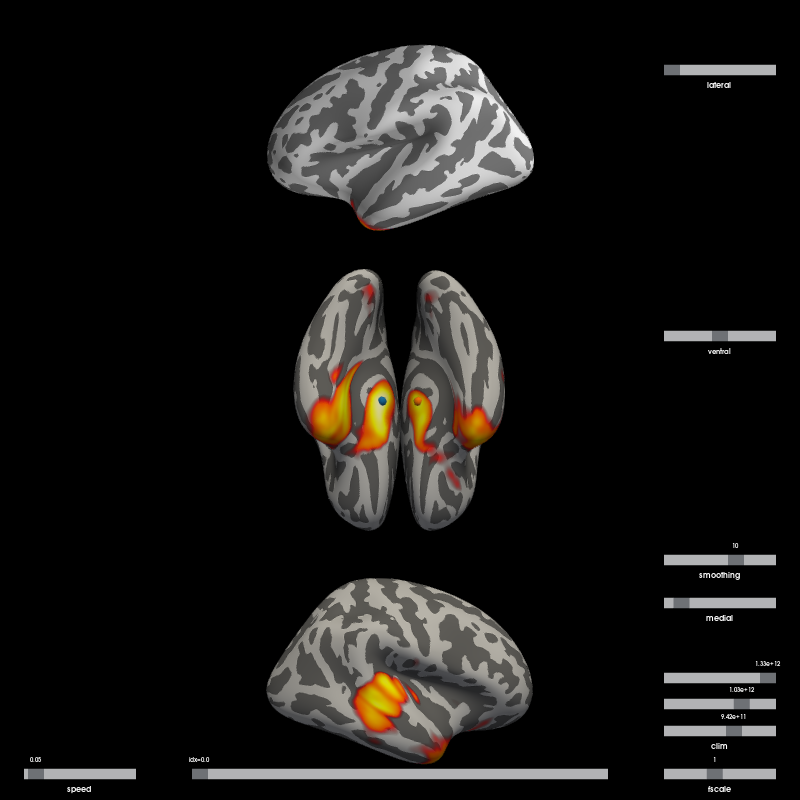
\includegraphics[width=0.4\textwidth]{./figures/amvica/amvica_camcan_montage_0.png}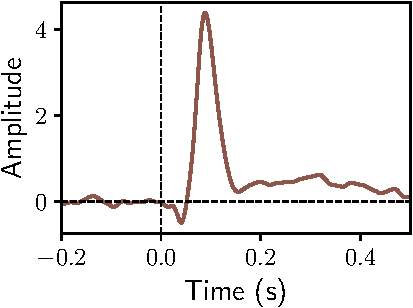
\includegraphics[width=0.4\textwidth]{./figures/amvica/amvica_camcan_source_0.pdf} \\
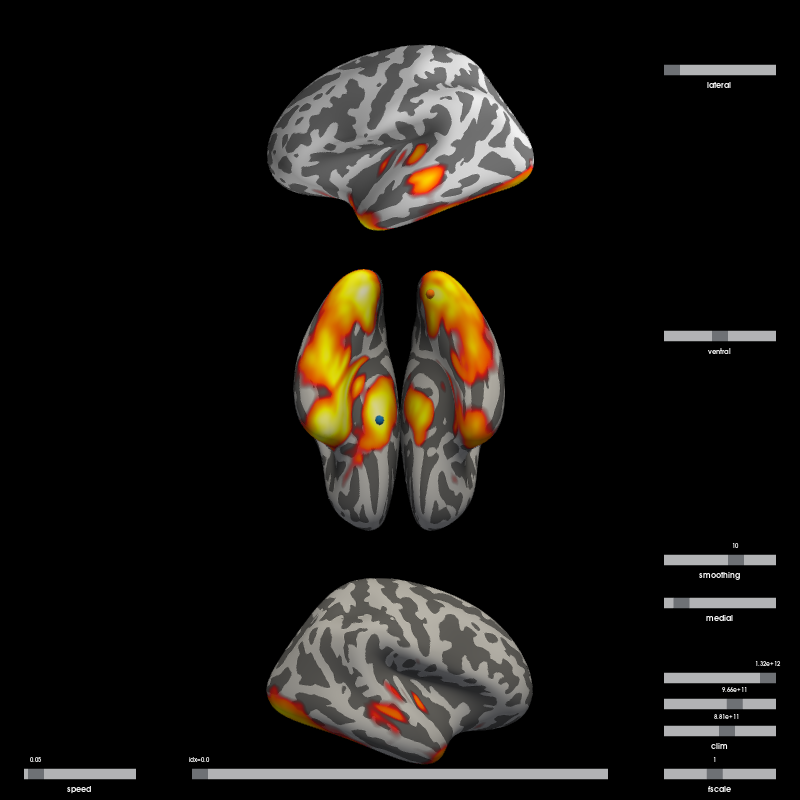
\includegraphics[width=0.4\textwidth]{./figures/amvica/amvica_camcan_montage_1.png}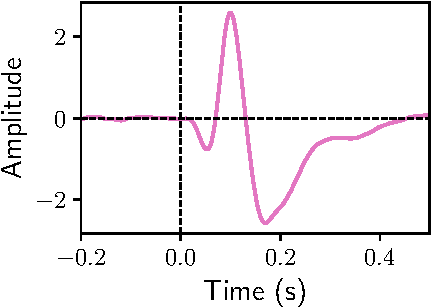
\includegraphics[width=0.4\textwidth]{./figures/amvica/amvica_camcan_source_1.pdf} \\
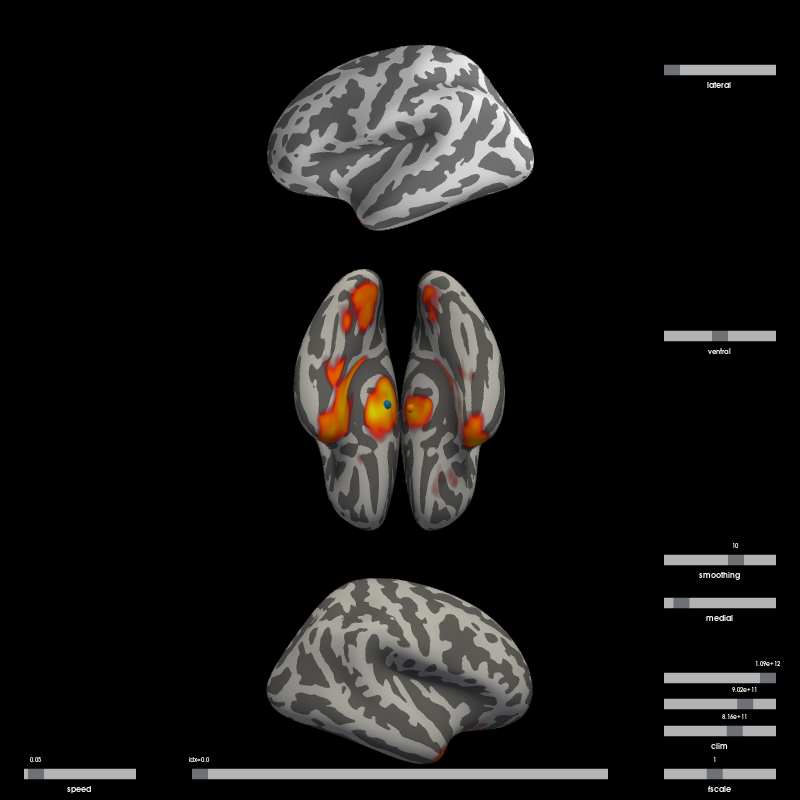
\includegraphics[width=0.4\textwidth]{./figures/amvica/amvica_camcan_montage_2.png}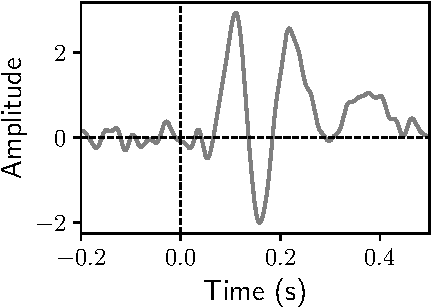
\includegraphics[width=0.4\textwidth]{./figures/amvica/amvica_camcan_source_2.pdf} \\
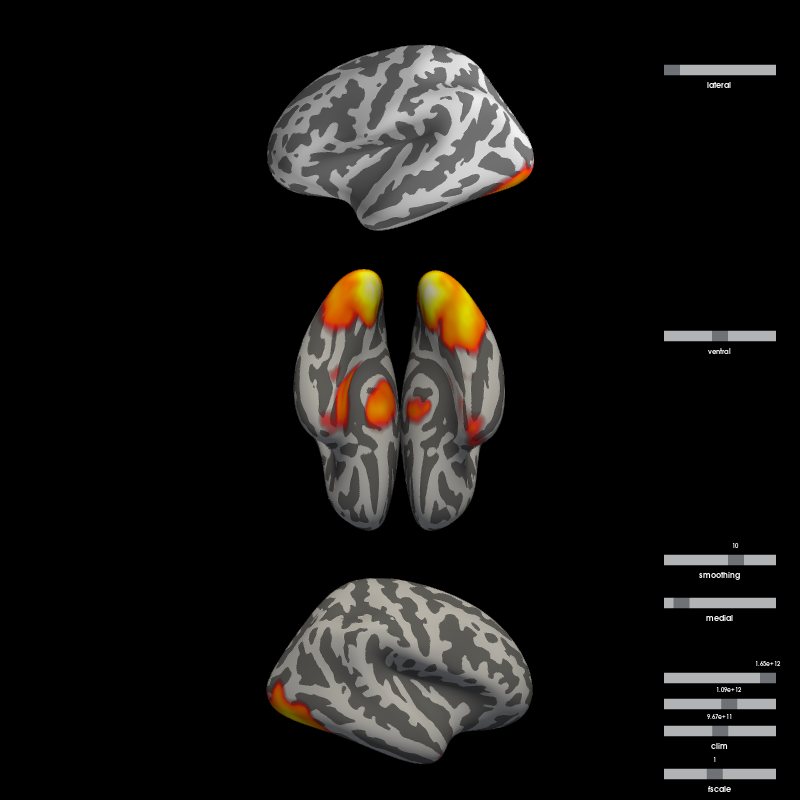
\includegraphics[width=0.4\textwidth]{./figures/amvica/amvica_camcan_montage_3.png}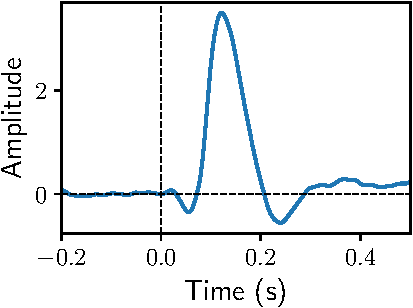
\includegraphics[width=0.4\textwidth]{./figures/amvica/amvica_camcan_source_3.pdf} \\
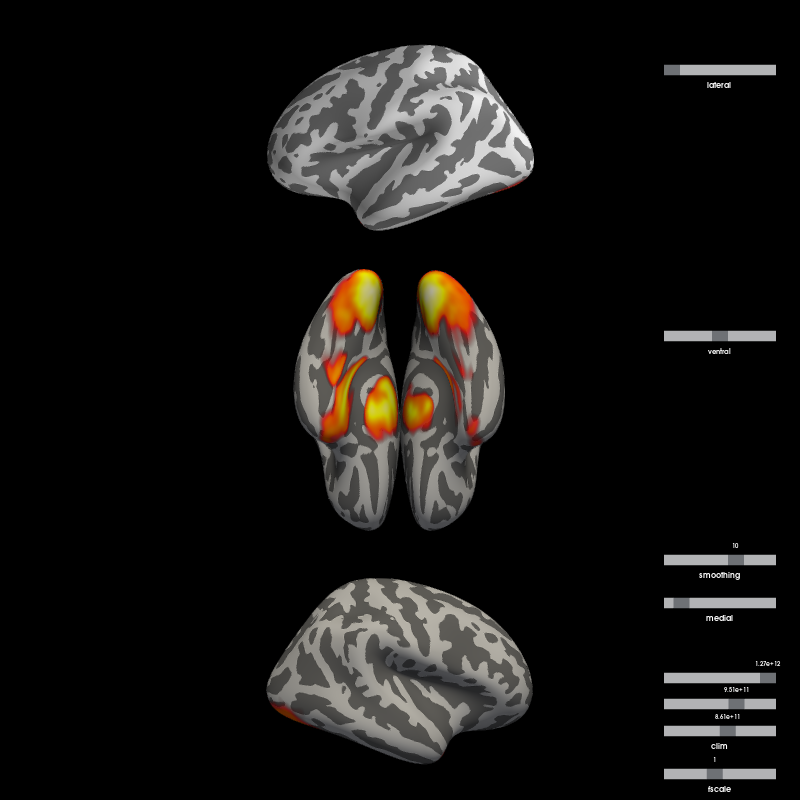
\includegraphics[width=0.4\textwidth]{./figures/amvica/amvica_camcan_montage_4.png}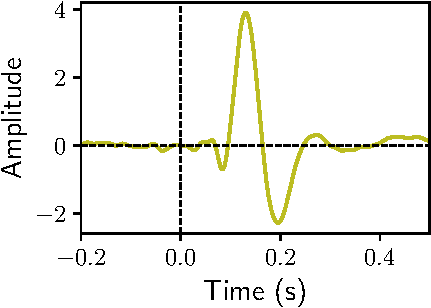
\includegraphics[width=0.4\textwidth]{./figures/amvica/amvica_camcan_source_4.pdf} \\
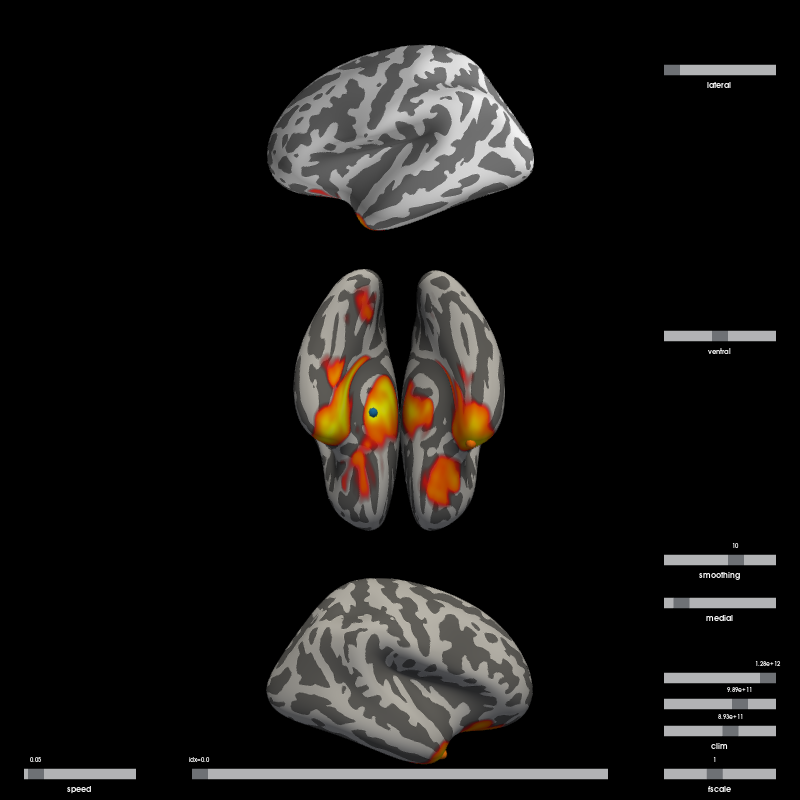
\includegraphics[width=0.4\textwidth]{./figures/amvica/amvica_camcan_montage_5.png}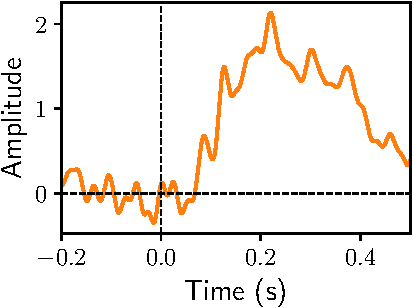
\includegraphics[width=0.4\textwidth]{./figures/amvica/amvica_camcan_source_5.pdf} \\
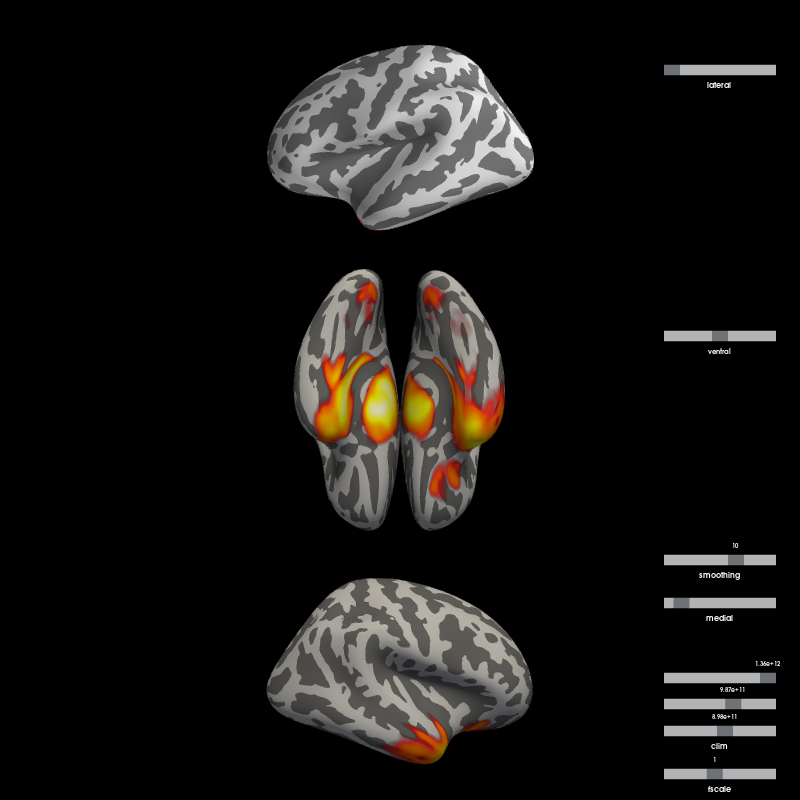
\includegraphics[width=0.4\textwidth]{./figures/amvica/amvica_camcan_montage_6.png}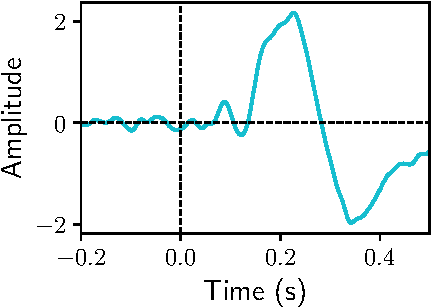
\includegraphics[width=0.4\textwidth]{./figures/amvica/amvica_camcan_source_6.pdf} \\
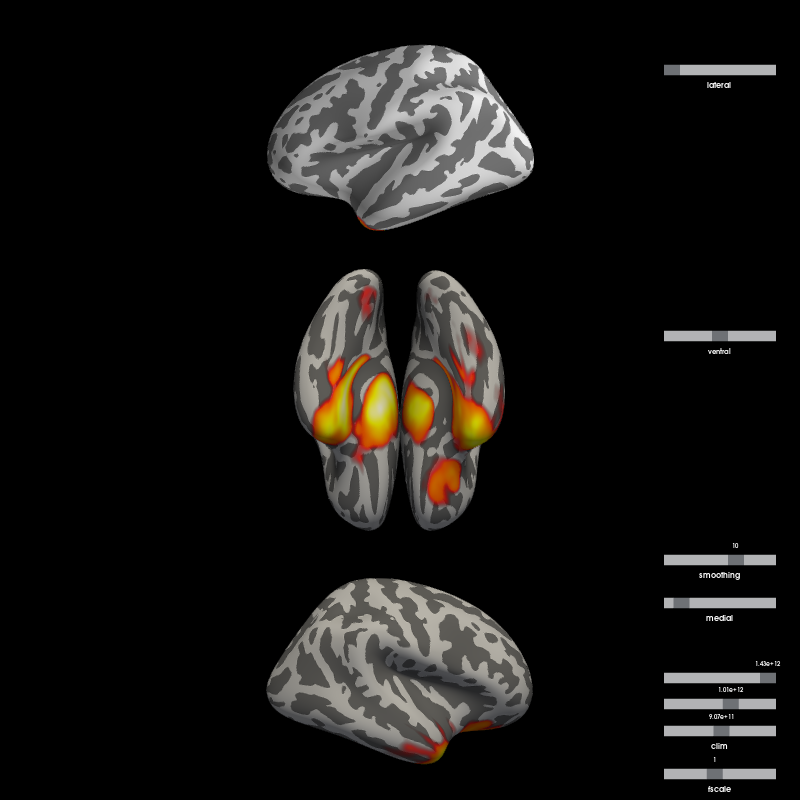
\includegraphics[width=0.4\textwidth]{./figures/amvica/amvica_camcan_montage_7.png}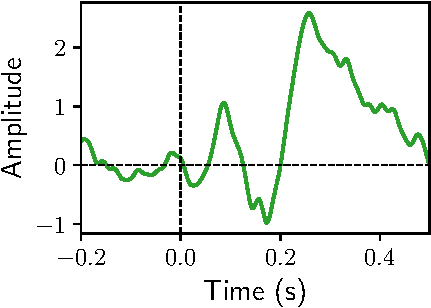
\includegraphics[width=0.4\textwidth]{./figures/amvica/amvica_camcan_source_7.pdf} \\
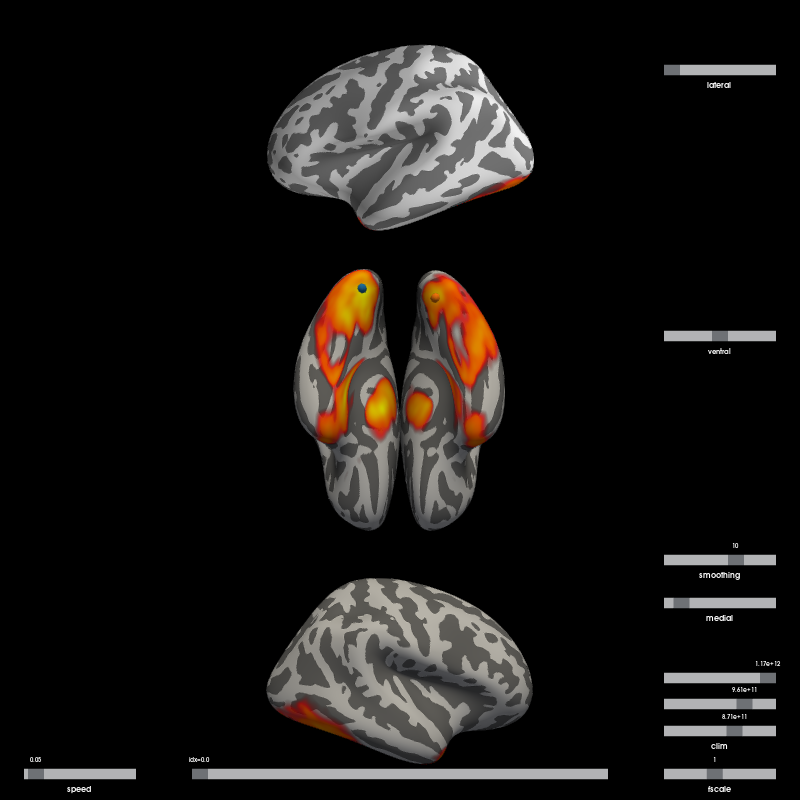
\includegraphics[width=0.4\textwidth]{./figures/amvica/amvica_camcan_montage_8.png}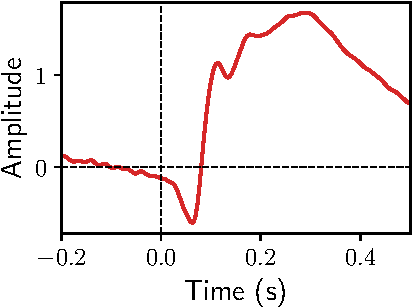
\includegraphics[width=0.4\textwidth]{./figures/amvica/amvica_camcan_source_8.pdf} \\
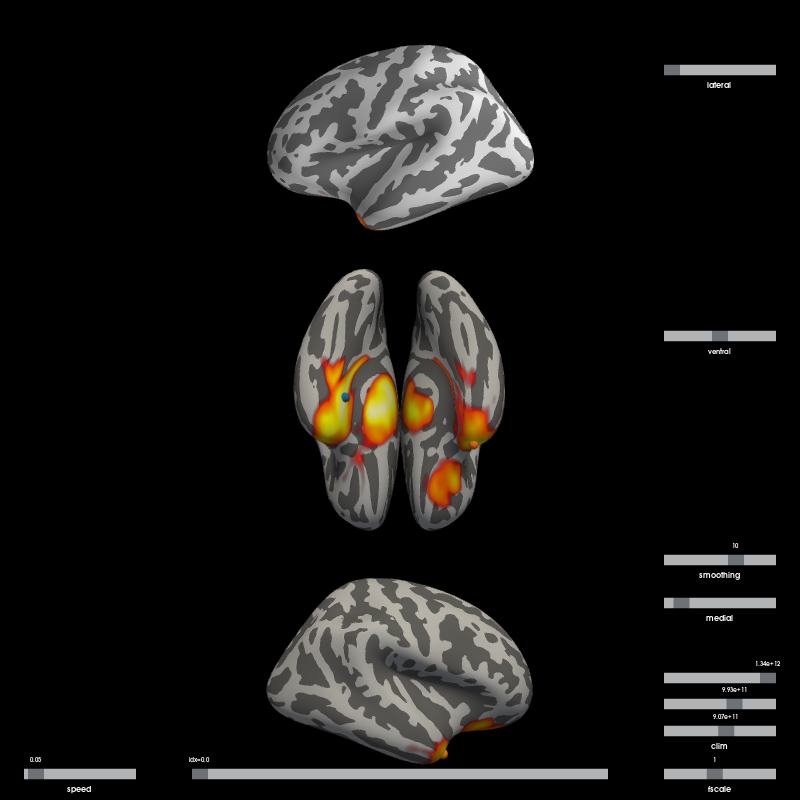
\includegraphics[width=0.4\textwidth]{./figures/amvica/amvica_camcan_montage_9.png}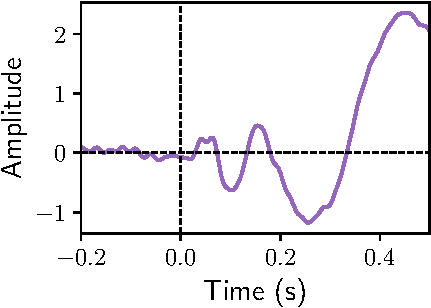
\includegraphics[width=0.4\textwidth]{./figures/amvica/amvica_camcan_source_9.pdf} \\
}